\documentclass[../main.tex]{subfiles}

\begin{document}

\section{Quantum getallen}%
\label{sec:quantum_getallen}

Er zijn verschillende quantum getallen die gebruikt worden. Deze kunnen opgesplitst worden in 2 groepen:
\begin{itemize}
    \item Additieve quantum getallen:
        \begin{itemize}
            \item baryon getal
            \item elektrische lading
            \item kleur
            \item lepton getal
            \item ...
        \end{itemize}
        Deze komen overeen met continue transformaties. Dit wil zeggen dat de getallen kunnen oplopen.
    \item Multiplicatieve kwantum getallen
        \begin{itemize}
            \item pariteit
            \item C-pariteit
            \item ...
        \end{itemize}
        Komen overeen met discrete transformaties en kunnen bv voor pariteit enkel -1 of 1 zijn.
\end{itemize}

\subsection{Elekrische lading}%
\label{sub:elekrische_lading}

We weten dat de elektrische lading behouden is.
\begin{equation}
    \begin{aligned}
        \label{eq:cons_lading}
        \sum_{init} Q_i = \sum_{final} Q_i
    \end{aligned}
\end{equation}
Dit wil zeggen dat de lichtste drager van de lading stabiel zal moeten zijn. Met een levensduur $\tau_e$ van het elektron groter dan $6.6\cdot 10^{28}$yr (90\% CL) is dit ook het geval.\\
De antideeltjes hebben tegengestelde lading.
\begin{equation}
    \begin{aligned}
        \label{eq:anti_deeltje_lading}
        |Q_{\epsilon^+}+Q_{\epsilon^-}|/e < 4\cdot 10^{-8}
    \end{aligned}
\end{equation}

\subsection{Lepton getal}%
\label{sub:lepton_getal}

Het lepton getal $\mathcal{L}$ is $+1$ voor de $e^-$, $\mu^-$, $\tau^-$ en de neutrino's en $-1$ voor $e^+$, $\mu^+$, $\tau^+$ en de antineutrino's. Voor al de andere deeltjes is het lepton getal $0$. Voor zover we weten is het lepton getal voor elke generatie behouden met een uitzondering van de neutrino oscillaties die dit niet behouden.\\
De som van de lepton getallen $\mathcal{L} = \mathcal{L}_e + \mathcal{L}_\mu + \mathcal{L}_\tau$ moet altijd behouden worden. Dit wil zeggen dat het lichtste neutrino moet stabiel zijn. Ergens weten we dat het lepton getal niet helemaal behouden kan zijn. Dit weten we \lq\lq zeker\rq\rq\  voor het baryon getal (zie hieronder).

\subsection{Baryon getal}%
\label{sub:baryon_getal}

Het baryon getal $\mathcal{B}$ is $+1$ voor al de baryonen, $-1$ voor al de anti-baryonen en $0$ voor de rest. In alles wat we ooit hebben gezien is het baryon getal behouden. Dit zegt ons terug dat het lichtste baryon, het proton, stabiel moet zijn. Met een levensduur  $\tau_p$ van meer dan $2.1\cdot 10^{29}$yr (90\% CL) is dat natuurlijk stabiel.\\
In de theorieën waar $\mathcal{B}$ niet behouden wordt, wordt $\mathcal{M}$ ook niet behouden. Maar wat er wel zou behouden worden worden is $\mathcal{B-L}$. Achter het behoud van deze 2 quantum getallen zit geen ijk principe. Dit zijn puur experimentele vaststellingen.  We weten dat deze niet helemaal behouden kunnen worden als we denken aan de big bang. Hier ontstaat het universum uit pure energie. Deze splitst op in deeltje-antideeltje paren. M.a.w. moet er bij de big bang even veel materie als anti-materie gecreerd zijn. Vandaag de dag nemen we deze anti-materie niet meer waar dus moet deze toch ergens verdwenen zijn.\\
De baryonen zijn opgesteld uit quarks en antiquarks. Dit geeft ons de nieuwe baryon getallen:
\begin{itemize}
    \item $\mathcal{B} = +\frac{1}{3}$ voor quarks
    \item $\mathcal{B} = -\frac{1}{3}$ voor antiquarks
    \item $\mathcal{B} = 0$ voor de rest
\end{itemize}

\subsection{Impuls moment}%
\label{sub:impuls_moment}

\begin{equation}
    \begin{aligned}
        \label{eq:impuls_moment}
        \vec{J}=\vec{L}+\vec{S}
    \end{aligned}
\end{equation}
Wat deze intrinsieke spin nu juist betekent, hangt af van de omstandigheden. We weten wel dat het totaal angulair moment behouden is. De fundamentele reden hiervoor is dat alles wat we zien en alle theorieën die we uitschrijven invariant zijn voor rotatie in de ruimte. Het behoud van energie komt uit de tijd invariatie en het behoud van moment uit de de ruimtelijke invariantie.\\
\begin{equation}
    \begin{aligned}
        \label{eq:samengesteld_moment}
        \vec{L} + \vec{S} &= \vec{J}\\
        |l-s| \leq &j \leq |l+s|\\
        j_3=m&=l_3+m_3
    \end{aligned}
\end{equation}
De angulaire moment operator is gegeven door:
\begin{equation}
    \begin{aligned}
        \label{eq:ang_mom_op}
        \hat{\vec{L}}^2&=l(l+1)\hbar^2\\
        \hat{L}_3&=l_3\hbar
    \end{aligned}
\end{equation}
Hierbij zijn de quantum getallen gegeven door $l=0,1,2...$ en $-l\leq l_3\leq l$. De angulaire momenta zullen veel samengesteld worden . Al de mogelijke combinaties van composities en decomposities worden gedaan aan de hand van de Clebsch-Gordan coëfficiënten. Die de kans tussen de verschillende quantum getallen zal weergeven. Zie hiervoor de oefeninglessen om goed mee te leren werken. De algebra van de Clebsch-Gordan coëfficiënten komt uit de symmetriegroep O(3), die isometrisch is met SU(2). 

\subsection{Strong isospin}%
\label{sub:strong_isospin}

We zien dat de Lagrangiaan van de sterke en zwakke interactie ijkinvariant is met als groep SU(2). Dit betekent dat het proton en neutron voor de sterke wisselwerking identiek zijn. Dit komt neer op het feit dat voor de sterke wisselwerking de up en down quark identiek zijn. Dit is niets anders dan het analogon voor een elektron met spin up $\left|e^\uparrow\right>$ en spin down $\left|e^\downarrow\right>$. Het proton en neutron vormen samen een sterk isospin doublet, de nucleonen:
\begin{equation}
    \begin{aligned}
        \label{eq:nucleonen}
        N = \binom{p}{n}
    \end{aligned}
\end{equation}
Een aantal verschillende sterke isospin multipletten zijn weergegeven in tabel \ref{tab:strong_isospin}. Hieruit lijkt dit een goed kwantum getal te zijn, omdat binnen een multiplet de deeltjes op een kleine afwijking na dezelfde massa te hebben. Het verschil in massa's binnen een multiplet komen van andere interacties, vooral de elektromagnetische. Omdat de massa's niet perfect overeen komen wil dit zeggen dat dit geen perfect kwantum getal zal zijn.

\begin{table}[h]
    \centering
    \caption{Strong isospin}
    \label{tab:strong_isospin}
    \begin{tabular}{c||cc|c|c|c|c}
                & $I$           & $I_3$         & $\mathcal{B}$ & $S$   & $Q$   & Mass (MeV)\\
        \hline
        $p$     & $\frac{1}{2}$ & $+\frac{1}{2}$& $1$           & $0$   & $+1$  & 938       \\
        $n$     & $\frac{1}{2}$ & $-\frac{1}{2}$& $1$           & $0$   & $0$   & 940       \\
        \hline
        $\pi^+$ & $1$           & $+1$          & $0$           & $0$   & $+1$  & 140       \\
        $\pi^0$ & $1$           & $0$           & $0$           & $0$   & $0$   & 135       \\
        $\pi^-$ & $1$           & $-1$          & $0$           & $0$   & $-1$  & 140       \\
        \hline
        $\eta$  & $0$           & $0$           & $0$           & $0$   & $0$   & 547       \\
        \hline
        $\Xi^0$ & $\frac{1}{2}$ & $+\frac{1}{2}$& $-2$          & $-2$  & $0$   & 1315      \\
        $\Xi^-$ & $\frac{1}{2}$ & $-\frac{1}{2}$& $-2$          & $-2$  & $-1$  & 1325      \\
    \end{tabular}
\end{table}

Naast de up en down quarks zijn er natuurlijk ook andere quarks ontdekt. Om deze toe te voegen is er een nieuw kwantumgetal toegevoegd, de hyperlading.
\begin{equation}
    \begin{aligned}
        \label{eq:hyperlading}
        I_3&=Q-\frac{Y}{2},& Y&=\mathcal{B}+S
    \end{aligned}
\end{equation}
Wetenschappers hadden de relatie tussen de sterke interactie en de elektromagnetische interactie ingezien. Later zijn er naast de lading, het baryon getal en de strangeness nog andere kwantum getallen voor de quarks gevonden. Deze zijn:

\begin{table}[h]
    \centering
    \label{tab:kwantum_getallen}
    \begin{tabular}{cccc}
        Strangeness & $S(s)=-1$ & $S(\overline s)=+1$   & $S(...)=0$    \\
        charm       & $C(c)=+1$ & $C(\overline c)=-1$   & $C(...)=0$    \\
        Bottomness  & $B(b)=-1$ & $B(\overline b)=+1$   & $B(...)=0$    \\
        Topness     & $T(t)=+1$ & $T(\overline t)=-1$   & $T(...)=0$
    \end{tabular}
\end{table}

en de hyperladig wordt uitgebreid tot:
\begin{equation}
    \begin{aligned}
        \label{eq:hyperlading_total}
        Y=\mathcal{B}+S+C+B+T
    \end{aligned}
\end{equation}
Hier zitten de $U$ en $D$ niet in omdat deze verwerkt zijn in $I_3$.\\
De sterke isospin zal behouden worden in de sterke interactie, $I_3$ is door zijn connectie met de lading $Q$ behouden in elektromagnetische interactie. Deze zijn niet behouden in de zwakke interactie.

\subsection{Multiplicatieve kwantum getallen}%
\label{sub:multiplicatieve_kwantum_getallen}

We kennen er 3:
\begin{itemize}
    \item $P$ pariteit
    \item $C$ pariteit: charge conjugation
    \item $T$ pariteit: time reversal
\end{itemize}
Het ``CPT-theorema'' is niets anders dan: Elke Lorentz invariante lokale kwantumveldentheorie is invariant onder CPT. De gemaakte assumpties om dit te bewijzen zijn:
\begin{itemize}
    \item Lorentz invariant
    \item Lokaliteit (geen interactie op afstand)
    \item Causaliteit (oorzaak voor effect)
    \item Het vacuum is de laagste energie toestand
    \item vlakke ruimte-tijd
    \item punt deeltjes
\end{itemize}
Als gevolg hebben we
\begin{equation}
    \begin{aligned}
        \label{eq:CPT_gevolgen}
        m_X&\equiv m_{\overline X}\\
        \Gamma_X&\equiv \Gamma_{\overline X}
    \end{aligned}
\end{equation}
Dit is bewezen in de experimenten: $|m_p-m_{\overline p}|<7\cdot10^{-10}$ (90\% CL).

\subsection{Pariteit}%
\label{sub:pariteit}

Spiegelen door de oorsprong.
\begin{equation}
    \begin{aligned}
        \label{eq:pariteit}
        \vec{r}&\rightarrow -\vec{r}\\
        \vec{p}&\rightarrow -\vec{p}\\
        \vec{L} = \vec{r}\times\vec{p}&\rightarrow -\vec{r} \times -\vec{p} = \vec{L}
    \end{aligned}
\end{equation}
Hier kan je duidelijk het verschil zien tussen een vector, $\vec{r}$ en $\vec{p}$, en een pseudo (axiale) vector, $\vec{L}$. Waarbij de vector van teken zal veranderen en de pseudo vector niet. Indien we 2 maal spiegelen door de oorsprong krijgen we de identiteit operator $P^2=1$ en kunnen we hieruit de eigenwaarden van $P$ bepalen, $\pm1$. $+1$ voor pseudo vectoren en $-1$ voor vectoren. De pariteit heeft de volgende eigenschappen:

\begin{table}[h]
    \centering
    \label{tab:par_eig}
    \begin{tabular}{r|rl}
        H-atoom             & $(-1)^l$                  &                   \\
        $\gamma$            & $-1$                      & uit Maxwell vgl.  \\
        $f\overline f,l=0$  & $-1$                      & uit Dirac vgl.    \\
        $f$                 & $+1$                      & conventie         \\
        $\overline f$       & $-1$                      & conventie         \\
        $f\overline f,l$    & $(-1)(-1)^l=(-1)^{l+1}$   &                   \\
        $b\overline b,l=0$  & $+1$                      &                   \\
        $b\overline b,l$    & $(-1)^l$                  &                   \\
    \end{tabular}
\end{table}

De reden waarom een foton een negatieve pariteit heeft komt uit de Maxwell vergelijkingen. Je kan dit inzien als je het elektrisch veld tussen een electron en positron bekijkt. Als deze door de oorsprong worden gespiegeld zal het teken van het elektromagnetische veld ook omdraaien.

\subsection{C-pariteit}%
\label{sub:c_pariteit}

Dit is het uitwisselen van de deeltjes met antideeltjes en omgekeerd. De eigentoestanden van de C operator zijn enkel de neutrale deeltjes (lading 0). Als voorbeeld, de C operator inwerkend op een proton geeft een antiproton, wat niet dezelfde deeltjes zijn. De eigenschappen van de C operator zijn:

\begin{table}[h]
    \centering
    \label{tab:c_eig}
    \begin{tabular}{r|r}
        $\gamma$        & $-1$          \\
        $n\gamma$       & $(-1)^n$      \\
        $b \overline b$, s=0 & $(-1)^{l}$  \\
        $b \overline b$ & $(-1)^{l+s}$  \\
        $f \overline f$ & $(-1)^{l+s}$  \\
    \end{tabular}
\end{table}

Bij het uitvoeren van de C operator op een boson-antiboson systeem en een fermion-antifermion systeem moeten we even nadenken. In de les werd het pion gebruikt als voorbeeld van een spin-0 deeltje. In de spin-uitwisseling van het meson-anitimeson systeem kunnen we zien dat er niets is veranderd aan de spin-golffuncties en het dus mogelijk is dat de pariteit enkel afhangt van $l$. Hetzelfde geldt ook voor boson-antiboson systemen.

\begin{figure}[h]
    \centering
    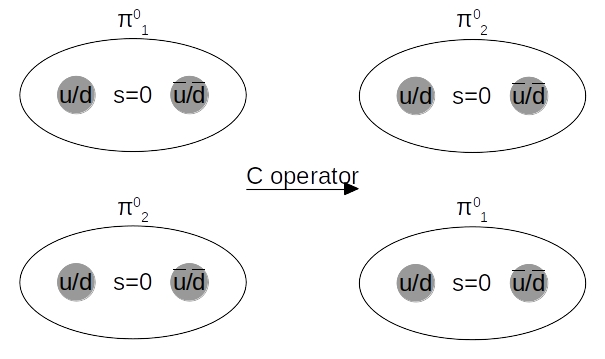
\includegraphics[width=0.8\linewidth]{quantum_numbers/baryon_c_operator.jpg}
    \caption{$\pi^0$ onder C operatie}%
    \label{fig:baryon_c_operator}
\end{figure}

Daarentegen kunnen de fermionen geen spin nul hebben. Als we kijken naar de verschillende combinaties die 2 fermionen kunnen ondergaan (figuur \ref{fig:fermion_c_operator}), zien we dat de spin golffunctie symmetrisch is voor $S$ oneven en antisymmetrisch voor $S$ even. Dit geeft ons voor de spin verrandering van 2 fermionen $(-1)^{s+1}$.

\begin{figure}[h]
    \centering
    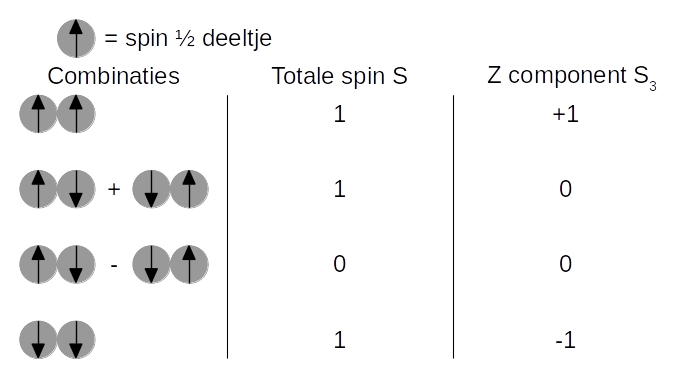
\includegraphics[width=0.8\linewidth]{quantum_numbers/fermion_c_operator.jpg}
    \caption{Fermion combinaties}%
    \label{fig:fermion_c_operator}
\end{figure}

\subsection{Pion pariteit}%
\label{sub:pion_pariteit}

Historisch gezien was het niet makkelijk om deeltjes uit elkaar te houden.
\begin{equation}
    \begin{aligned}
        \label{eq:pion_mass}
        \mu^\pm &\simeq 105 \text{MeV}\\
        \pi^\pm &\simeq 140 \text{MeV}\\
        \pi^0   &\simeq 135 \text{MeV}\\
    \end{aligned}
\end{equation}
Deze deeltjes zijn ontdekt in kosmische straling. Het verschil tussen het muon en de pions is dat het muon een lepton is en dus enkel elektromagnetisch interageert. Bij het onderzoek gaven de muonen in de gaskamer een mooie lijn van geïoniseerd gas en de pionen een knal. In die tijd kon geen onderscheid gemaakt worden tussen de massa van de 2 deeltjes. Wat wel makkelijk te herkennen was waren $\pi^0$ die vervallen in 2 fotonen. Door de energie van de 2 fotonen samen te tellen krijg je perfect een piek bij $135$MeV. Omdat $\gamma$ een spin 1 deeltje is en dat het pion vervalt in 2 $\gamma$'s weten we dat $\pi^0$ een boson moet zijn. Het moet een heeltallige spin hebben om te kunnen vervallen in 2 $\gamma$'s. Of er een relatie was tussen $\pi^\pm$ en $\pi^0$ en dus ook een verschil tussen $\mu$ en $\pi^\pm$ heeft een lange tijd geduurd. De spin van $\pi^0$ is bepaald aan de hand van de vervallen $\gamma+\gamma$ en $e^++e^-+e^++e^-$ die uitgezet zijn in Dalitz plots. Zo bekomen we experimenteel dat de totale spin voor de pionen $J=0$ is.\\
Het bepalen van de pariteit van pionen kan gedaan worden aan de hand van het volgende experiment:
\begin{equation}
    \begin{aligned}
        \label{eq:pion_pariteit}
        \pi^- + d \rightarrow n + n
    \end{aligned}
\end{equation}
Een $\pi^-$ bundel kan bekomen worden door een protonenbundel in te sturen op een blok materie en door een spectroscoop de $\pi^-$ deeltjes af te zonder van de rest. Deze laag energetische pionen verliezen in $D_2O$ energie en kunnen ingevangen worden in deuterium. Deze hoog aangeslagen toestanden zenden X-stralen uit tot ze in de grondtoestand terug vallen.
\begin{equation}
    \begin{aligned}
        \label{eq:grondtoestand_deuteron}
        s_d=1\text{; }s_\pi=0 \Rightarrow J=1
    \end{aligned}
\end{equation}
De reden waarom $L=0$ is in dit geval is omdat het samengesteld systeem zich in de grondtoestand bevindt (S-state). De spin van het deuterium kan eigenlijk $0$ of $1$ zijn. De reden waarom het onmogelijk is om een $s_d=0$ te hebben kunnen we vinden door de symmetrie van de golffunctie van het deuterium ($D=p+n$) te bekijken (behoud angulair moment).

\begin{table}[h]
    \centering
    \caption{Symmetrie van deuterium golffunctie}
    \label{tab:sym_deut_golf}
    \begin{tabular}{cccc}
        $\psi_f\sim$ & $\phi(r)$ & $\chi(s)$                & $\Psi(I)$             \\
        $-$             & $+$       & {\color{green} $+$}   & {\color{green} $-$}   \\
        $-$             & $+$       & {\color{red} $-$}     & {\color{red} $+$}     \\
    \end{tabular}
\end{table}

De golffunctie van het deuteron moet negatief zijn voor de omwisseling van het proton en neutron. Omdat we $L=0$ hebben is het ruimtelijke orbitaal altijd symmetrisch. De spin kan zowel symmetrisch als antisymmetrisch zijn met de isospin het tegengestelde omdat anders de antisymmetrie van de symmetrie niet correct is. De verschillende spin en isospin op mengingen zijn gegeven door:

\begin{table}[h]
    \centering
    \caption{Multipletten van deuterium}
    \label{tab:mult_deut}
    \begin{tabular}{cc}
        spin multiplet & isospin multiplet \\
        {\color{green} $\uparrow\uparrow$, $\downarrow\downarrow$, $\uparrow\downarrow+\downarrow\uparrow$} & {\color{green} $np-pn$} \\
        {\color{red} $\uparrow\downarrow-\downarrow\uparrow$} & {\color{red} $nn$, $pp$, $np+pn$}
    \end{tabular}
\end{table}

Experimenteel zien we dat de $nn$ en $pp$ niet bestaan. Enkel het isospin singlet bestaat en $s_d$ moet dus $1$ zijn.\\
Nu we weten wat de spin is van de begin toestanden kunnen we dat ook doen voor de eind toestanden. De spin van neutronen is $1/2$ en hebben we dus 2 mogelijkheden voor de totale spin van $0$ of $1$. De symmetrie van het neutron-neutron paar is gegeven door $(-1)^{S+1}$, wat hetzelfde is als in tabel \ref{tab:sym_deut_golf} voor het deuterium geval. We weten ook dat als we de 2 neutronen uitwisselen met elkaar dan weten we dat de volledige symmetrie van de golffunctie negatief moet zijn $\Rightarrow (-1)^{L+S+1}=-1$ (Pauli principe). Dit wil zeggen dat dat $L+S$ voor de neutronen even moet zijn. Er zijn 3 mogelijkheden om $\vec{J}=\vec{L}+\vec{S}$ van de neutronen gelijk aan $1$ te krijgen.
\begin{itemize}
    \item $L=0$, $S=1$
    \item $L=1$, $S=0,1$
    \item $L=2$, $S=1$
\end{itemize}
Hiervan is uiteindelijk maar 1 combinatie waar $L+S$ even is: $L=1$, $S=1$, al de andere zijn oneven. Met andere woorden moeten de 2 neutronen hun spin parallel staan en in een P-golf rond elkaar bewegen. De uiteindelijke toestand van de neutronen kunnen neergeschreven worden als $^3P_1$ met een pariteit $(-1)^L = -1$. Nu kan je je afvragen wat het verschil is tussen deze symmetrie en de eerder gegeven symmetrie $(-1)^{L+S+1}$. $(-1)^{L+S+1}$ is de symmetrie van de totale golffunctie van het neutron-neutron paar (altijd antisymmetrisch voor fermionen) en $(-1)^L$ is de symmetrie onder spiegeling rond de oorsprong.\\
Omdat protonen en neutronen dezelfde intrisieke pariteit hebben hangt de pariteit van deuterium enkel af van het baanmoment tussen $p$ en $n$. Omdat $L_d=0$ hebben we uiteindelijk dat $P_d=(-1)^0=+1$.\\
Met al deze gegevens kunnen we nu de pariteit van $\pi^-$ bepalen. Uit behoud van pariteit kunnen we halen dat de pariteit van $\pi^-+d$ gelijk moet zijn aan $-1$. Vul dit allemaal in en dan vinden we:
\begin{equation}
    \begin{aligned}
        \label{eq:par_pi_-}
        P_\pi\cdot P_d\cdot (-1)^{L_{\pi+d}} &\rightarrow p_\pi\cdot (+1) \cdot (+1) = -1\\
                                             &\Rightarrow P_\pi=-1
    \end{aligned}
\end{equation}

\subsection{$G$-pariteit}%
\label{sub:g_pariteit}

De reden dat dit is ingevoerd is omdat de $C$ operator enkel een goed kwantum getal voor $Q=0$. Een uitbreiding van de C operator is de $G$ operator die de tekortkomingen van de $C$ operator zou moeten opvangen.
\begin{equation}
    \begin{aligned}
        \label{eq:g_operator}
        G=CR=C\exp(i\pi I_2)
    \end{aligned}
\end{equation}
De $R$ operator is een rotatie over $180^\circ$ over de isospin y-as. In figuur \ref{fig:pi_g_operator} kan je zien hoe deze operator zal inwerken op een $\pi^+$.

\begin{figure}[h]
    \centering
    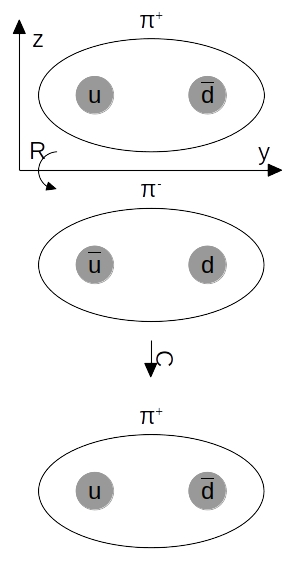
\includegraphics[width=0.4\linewidth]{quantum_numbers/pi_g_operator.jpg}
    \caption{$G$ operator inwerkend op een pion}%
    \label{fig:pi_g_operator}
\end{figure}

Kijken we naar de eigentoestanden van de $R$ operator zien we voor de ruimtelijke sferische golffunctie (rotatie $180^\circ$ rond y-as, $\exp(i\pi L_y$):
\begin{equation}
    \begin{aligned}
        \label{eq:ruimte_y_rotatie}
        Y_l^0(\theta, \phi) \rightarrow Y_l^0(\pi - \theta, \pi - \phi) = (-1)^lY_l^0
    \end{aligned}
\end{equation}
Het equivalent kan gedaan worden voor de isospin golffunctie $I_3=0$:
\begin{equation}
    \begin{aligned}
        \label{eq:isospin_y_rotatie}
        \chi(I,0) \rightarrow (-1)^I\chi(I,0)
    \end{aligned}
\end{equation}
De eigenwaarde voor de $R$ operator is dus $(-1)^I$. De reden waarom de z component van de isospin $0$ mag genomen worden is omdat deze toch behouden wordt door de sterke wisselwerking en dus geen verschil zou maken als we die anders kiezen. Voegen we dit samen met dit voor de $C$ operator krijgen we de eigenwaarde van de $G$ operator:
\begin{equation}
    \begin{aligned}
        \label{eq:eigenwaarde_g}
        G\left|\psi\right>=(-1)^{l+s+I}\left|\psi\right>
    \end{aligned}
\end{equation}
Terug voor $\pi^0$ hebben we:
\begin{itemize}
    \item $C=+1$ door het verval $\pi^0\rightarrow2\gamma$ waarbij de pariteit van 2 gelijke deeltjes altijd positief zal zijn
    \item $R=(-1)^1=-1$
\end{itemize}
Dit samen geeft $G\left|\pi\right>=-\left|\pi\right>$. Dit geld voor alle pionen omdat de sterke lading niet naar de lading kijkt. Hieruit kunnen we ook halen dat $G\left|n\pi\right>=(-1)^n\left|n\pi\right>$.\\
Een mooi voorbeeld waar deze $G$ operator te pas komt is bij de het verschil tussen $\rho(780\text{MeV})$ en $\omega(780\text{MeV})$. Deze hebben beide een immense verval breedte en kunnen zou dus niet uit elkaar gehouden worden. Het enige verschil is dat $I_\rho=1$ en $I_\omega=0$ met respectievelijk $G_\rho=+1$ en $G_\omega=-1$. Zo zien we dat $\rho$ zal vervallen naar 2 pionen en $\omega$ naar 3. Zo is het mogelijk om deze bij een experiment uit elkaar te houden.\\
Meestal zullen mesonen als volgt voorgesteld worden: $I^G(J^{PC})$. Belangrijk om te weten is dat de $G$ pariteit enkel behouden wordt door de sterke wisselwerking.\\

{\color{red} mogelijke examenvraag: aantal mesonen gegeven, leid de isospin, spin, pariteit ($=(-1)^{L+1}$ extra - teken door tegengestelde intrinsieke pariteit)... af uit de toestand}

\end{document}
